\documentclass[border=10pt]{standalone}

\usepackage{tikz}
\usepackage{tikzsymbols}
\usetikzlibrary{calc,patterns,shapes.geometric}

\def\centerarc[#1](#2)(#3:#4:#5){\draw[#1] ($(#2)+({#5*cos(#3)},{#5*sin(#3)})$) arc (#3:#4:#5);}

\begin{document}
	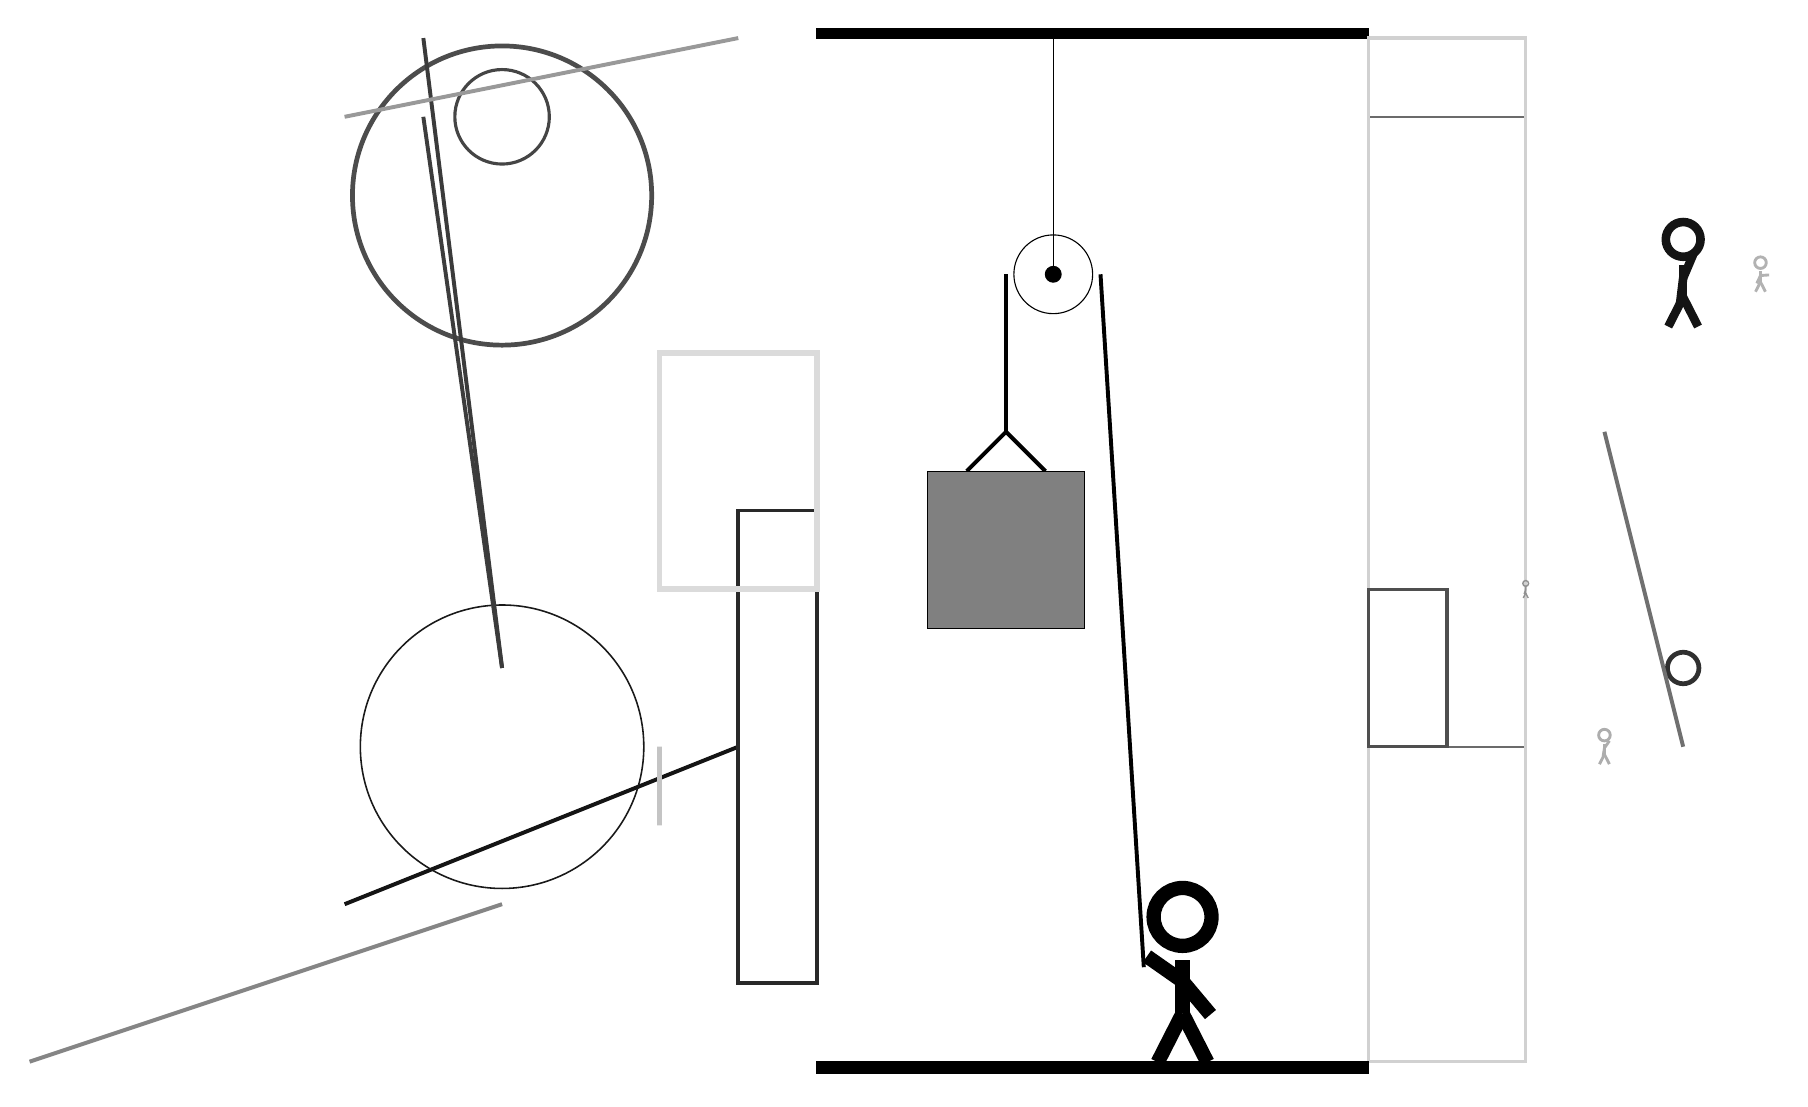
\begin{tikzpicture}
		%%%%% START %%%%%
		
		\draw[fill=black] (-2, 10) rectangle (5, 10.125);
		
		\draw (1, 7) circle (0.5);
		\draw[fill=black] (1, 7) circle (0.1);
		\draw (1, 10) -- (1, 7);
		
		\draw[line width=0.5mm, color=black!92](-3, 1) -- (-8, -1);
		
		\node[line width=0.7mm, color=black!92] at (9, 7) {\Strichmaxerl[6][83][67]};
		\node[line width=0.4mm, color=black!32] at (8, 1) {\Strichmaxerl[2][81][55]};
		\draw [line width=0.6mm, color=black!70](-6, 8) circle (1.9);
		\draw[line width=0.5mm, color=black!84] (-3, -2) rectangle (-2, 4);
		\draw[line width=0.7mm, color=black!14] (-4, 6) rectangle (-2, 3);
		
		\draw [line width=0.6mm, color=black!81](9, 2) circle (0.2);
		\draw[line width=0.5mm, color=black!56](8, 5) -- (9, 1);
		\draw[line width=0.2mm, color=black!58] (5, 9) rectangle (7, 1);
		
		\draw[line width=0.4mm, color=black!18] (5, -3) rectangle (7, 10);
		\draw[line width=0.6mm, color=black!23] (-4, 1) rectangle (-4, 0);
		
		\draw [line width=0.2mm, color=black!90](-6, 1) circle (1.8);
		\node[line width=0.3mm, color=black!30] at (10, 7) {\Strichmaxerl[2][65][4]};
		
		\draw[line width=0.5mm, color=black!76](-6, 2) -- (-7, 9);
		\draw[line width=0.4mm, color=black!69] (5, 3) rectangle (6, 1);
		\draw[line width=0.5mm, color=black!48](-6, -1) -- (-12, -3);
		
		\draw [line width=0.4mm, color=black!73](-6, 9) circle (0.6);
		\draw[line width=0.5mm, color=black!77](-7, 10) -- (-6, 2);
		\draw[line width=0.5mm, color=black!40](-3, 10) -- (-8, 9);
		
		\node[line width=0.7mm, color=black!43] at (7, 3) {\Strichmaxerl[1][69][89]};
		
		\draw[line width=0.5mm] (-0.1, 4.5) -- (0.4, 5.0) -- (0.9, 4.5);
		\draw[fill=black!50] (-0.6, 4.5) rectangle (1.4, 2.5);
		
		\draw[line width=0.5mm] (0.4, 7) -- (0.4, 5.0);
		\centerarc[line width=0.5mm](1, 7)(0:180:0.6);
		\draw[line width=0.5mm](1.6, 7) -- (2.15, -1.8);
		
		\node at (2.6, -1.9) {\Strichmaxerl[10][-35][-50]};
		
		\draw[fill=black] (-2, -3) rectangle (5, -3.15);
		
		%%%%% END %%%%%
	\end{tikzpicture}
\end{document}